\section{Kameramodell}
Da das verwendete Fisheye-Objektiv durch seinen großen Blickwinkel stark verzerrt auf den Kamerasensor abbildet, ist eine spezielles Kameramodell zur Rektifizierung der Bilddaten notwendig. Wir haben uns in dieser Arbeit für die Nutzung einer Matlab-Toolbox entschieden  \autocite{OCamCalibOmnidirectionalCamera, scaramuzzaFlexibleTechniqueAccurate2006, scaramuzzaToolboxEasilyCalibrating2006, scaramuzzaOmnidirectionalVisionCalibration2007, rufliAutomaticDetectionCheckerboards2008}. Das in selbiger verwendete Modell und die Anwendung dessen zur Rektifizierung soll nun erleutert werden. 

Die OcamCalib-Toolbox behandelt das Kamerasystem als Einheit, d.h. die Kamera und der Fisheyeobjektivaufsatz (alternativ der konvexe Spiegel) werden zusammen durch einen Parametersatz beschrieben.

Das Modell hat das Ziel, den Zusammenhang zwischen einem Punkt auf dem Bildsensor \gls{lat:camerapoint} mit Koordinaten (u,v) und einem vom optischen Zentrum des Objektivs ausgehenden Vektors nicht festgelegter Länge \gls{lat:cameravector} mit Koordinaten (x,y,z) zu finden.

\begin{figure}[htb]
  \centering
  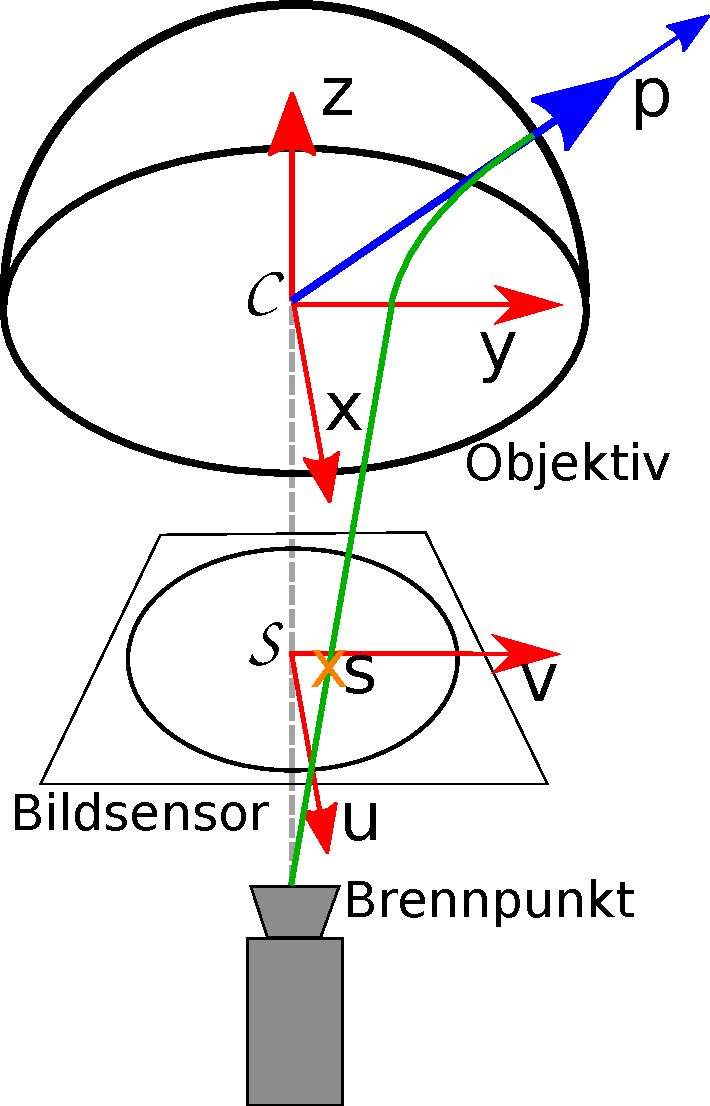
\includegraphics[width=0.5\textwidth]{OCamCalib_Kameramodell}
  \caption{Das Kameramodell der OCamCalib Toolbox}
  \label{fig:kameramodell}
\end{figure}

\subsection{Annahmen}
Im verwendeten Modell werden folgende annahmen gemacht:
\begin{itemize}
\item Die verwendete Optik stellt ein zentrales Kamersystem dar, d.h. alle einfallendenden Lichtstrahlen treffen sich in einem Punkt. Dies ist der Koordinatenursprung des Kamerakoordinatensystems XYZ
\item Studienarbeiten
\item Diplomarbeiten
\item Praktikumsberichte
\end{itemize}

Da ein Darlegen des Prozesses zur Ermittlung der Parameter den Rahmen dieser Arbeit sprengen würde, wird darauf verzichtet.